\section{Introdução}\label{intro}
Esse relatório descreve a reprodução do experimento de Thomas Young proposta para a disciplina de Física Moderna da Faculdade UnB-Gama. Visa assim mostrar propriedades de onda que a luz possui, e colher dados experimentais para análise, sendo realizado da seguinte forma: Confecção de fendas para difração, confecção do circuito que possibilita utilizar um sensor (LDR), leitura do sensor para um microcontrolador e em seguida leitura e tratamento dos dados na porta serial do computador.

Se a luz consistisse estritamente de  partículas  normais ou clássicas, e estas partículas fossem disparadas em linha reta através de uma fenda e deixa-se chegar a uma superfície, do outro lado, seria de esperar um padrão correspondente ao tamanho e à forma da fenda. No entanto, quando esta "experiência de única fenda" é efectivamente realizado, o padrão na superfície (parede) é um padrão de difração em que a luz se espalha. Quanto menor a fenda, maior o angulo de dissipação.

Da mesma forma, se a luz consistisse de partículas estritamente clássicas e iluminado duas fendas paralelas, o padrão esperado na superfície seria simplesmente a soma das duas fendas de um único padrão. Na realidade, porém, o padrão muda para uma série de faixas claras e escuras. Quando Thomas Young demonstrou pela primeira vez este fenômeno, indicou que a luz consiste de ondas, já que a distribuição de brilho pode ser explicada pela interferencia construtiva e interferência destrutiva de frentes de onda. A experiência de Young, realizada no início de 1800, desempenhou um papel vital na aceitação da teoria ondulatória da luz, vencendo a teoria corpuscular da luz, proposta por Isaac Newton, que tinha sido o modelo aceito de propagação da luz nos séculos 17 e 18. No entanto, a descoberta posterior do efeito fotoeléctrico demonstrou que, em função das circunstâncias, a luz pode comportar-se como se ela fosse composta de partículas discretas. Estas descobertas aparentemente contraditórias tornou necessário ir além da física clássica e tomar a natureza quântica da luz em conta.

\subsection{Dualidade}\label{dualidade}

A teoria quântica nos diz que tanto a luz quanto a matéria consistem de pequenas partículas que apresentam propriedades semelhantes à das ondas. A luz é composta de partículas chamadas de fótons e a matéria é composta de partículas chamadas de elétrons, prótons, nêutrons. É só quando a massa de uma partícula fica pequena o suficiente que suas propriedades ondulatórias aparecem.

Com o experimento feito por Thomas Young percebemos propriedades de onda na luz, sendo essas a difração e interferência:

\begin{figure}[H]
\begin{center}
\begin{tikzpicture}[decoration=penciline, decorate,scale=1]
	\draw[thick] (0,0) -- (0,2.4) ; % barra de baixo
	\draw[thick] (0,2.6) -- (0,5) ; % barra de cima
	\draw[thick] (3,0) -- (3,5) ; % barra de choque
	\draw[line] (-1,2.5) -- (-0.2,2.5) ; % barra de choque
	% ondas primarias
	\foreach \A in {0,0.1,0.2,0.3,0.4,0.5} {
		\draw[thick] (-0.8 + \A,2) -- (-0.8 + \A,3) ;
	}
	\node[black,scale=0.4] at (-0.6,1.8) {$\overbrace{\text{Ondas incidentes}}$};
	% ondas após a fenda
	\foreach \A in {0,0.2,0.4,0.6,0.8,1,1.2,1.4} {
		\draw[thick] (0.2+\A,2.0-\A) -- (0.2+\A,2.01-\A) arc (-70:70:0.5+\A) ;
	}
\end{tikzpicture}
\end{center}
\caption{Difração em fenda simples}
\label{diff_simples}
\end{figure}

%--------------------------------
\begin{figure}[H]
\begin{center}
\begin{tikzpicture}[decoration=penciline, decorate,scale=1]
	\draw[thick] (0,0) -- (0,2.2) ; % barra de baixo
	\draw[thick] (0,2.4) -- (0,2.6) ; % barra de baixo
	\draw[thick] (0,2.8) -- (0,5) ; % barra de cima
	\draw[thick] (3,0) -- (3,5) ; % barra de choque
	\draw[line] (-1,2.5) -- (-0.2,2.5) ; % barra de choque
	% ondas primarias
	\foreach \A in {0,0.1,0.2,0.3,0.4,0.5} {
		\draw[thick] (-0.8 + \A,2) -- (-0.8 + \A,3) ;
	}
	\node[black,scale=0.4] at (-0.6,1.8) {$\overbrace{\text{Ondas incidentes}}$};
	% ondas após a fenda
	\foreach \A in {0,0.2,0.4,0.6,0.8,1,1.2,1.4} {
		\draw[thick,color=red] (0.02+\A,2-\A) -- (0.02+\A,2.01-\A) arc (-85:85:0.3+\A) ;
	}
	% ondas após a fenda
	\foreach \A in {0,0.2,0.4,0.6,0.8,1,1.2,1.4} {
		\draw[thick,color=green] (0.02+\A,2.4-\A) -- (0.02+\A,2.41-\A) arc (-85:85:0.3+\A) ;
	}
	% colisão das ondas
	\draw[dashed,->] (0.3,2.2) -- (10:3.5cm) ; % colisão 1
	\draw[dashed,->] (0.31,2.81) -- (52:5.5cm) ; % colisão 2
	\draw[dashed,->] (0.3,2.5) -- (35:4.3) ; % colisão 3
	
	\node[black,scale=0.4] at (4.05,4.35) {Colisão das ondas};
	\node[black,scale=0.4,align=left] at (4.25,2.46) {Colisão das ondas\\ com maior intensidade};
	\node[black,scale=0.4] at (4.1,0.55) {Colisão das ondas};
\end{tikzpicture}
\end{center}
\caption{Difração em fenda dupla (com interferência)}
\label{diff_dupla}
\end{figure}

Mesmo que a luz seja composta de partículas chamadas fotons, pode-se facilmente mostrar que a luz pode ser considerada uma onda electromagnética que se propaga com a velocidade da luz. A frequência da luz está relacionada com o seu comprimento de onda de acordo com

\begin{equation}\label{frequencia}
	f= \frac{C}{\lambda}
\end{equation}

Sendo $C$ a velocidade da luz, $\lambda$ o seu comprimento de onda, e $f$ a frequência.

Pode parecer bastante óbvio que a luz se comporta como uma onda, mas a prova de que a luz é realmente composta de partículas vem da experiência do efeito fotoelétrico.

\begin{figure}[H]
\begin{center}
\begin{tikzpicture}[decoration=penciline, decorate,scale=1]
	\draw[thick] (0,0) -- (0,2) ; % lado esquerdo
	\draw[thick] (0,2) -- (2,2) ; % lado superior
	\draw[thick] (2,2) -- (2,0) ; % lado direto
	\draw[thick] (2,0) -- (0,0) ; % lado inferior
	\draw[thick,->] (0,5) -- (1,2) ; % colisão luz
	\node[black,scale=0.8] at (0,5.2) {light};
	\node[black,scale=0.8] at (0.2,0.2) {$e⁻$};
	\node[black,scale=0.8] at (0.4,0.2) {$e⁻$};
	\node[black,scale=0.8] at (0.6,0.2) {$e⁻$};
	\node[black,scale=0.8] at (0.8,0.2) {$e⁻$};
	\node[black,scale=0.8] at (1.0,0.2) {$e⁻$};
	\node[black,scale=0.8] at (1.2,0.2) {$e⁻$};
	\node[black,scale=0.8] at (1.4,0.2) {$e⁻$};
	\node[black,scale=0.8] at (1.6,0.2) {$e⁻$};
	\node[black,scale=0.8] at (1.8,0.2) {$e⁻$};
	
	\node[black,scale=0.8] at (0.2,0.4) {$e⁻$};
	\node[black,scale=0.8] at (0.4,0.4) {$e⁻$};
	\node[black,scale=0.8] at (0.6,0.4) {$e⁻$};
	\node[black,scale=0.8] at (0.8,0.4) {$e⁻$};
	\node[black,scale=0.8] at (1.0,0.4) {$e⁻$};
	\node[black,scale=0.8] at (1.2,0.4) {$e⁻$};
	\node[black,scale=0.8] at (1.4,0.4) {$e⁻$};
	\node[black,scale=0.8] at (1.6,0.4) {$e⁻$};
	\node[black,scale=0.8] at (1.8,0.4) {$e⁻$};
	
	\node[black,scale=0.8] at (0.2,0.6) {$e⁻$};
	\node[black,scale=0.8] at (0.4,0.6) {$e⁻$};
	\node[black,scale=0.8] at (0.6,0.6) {$e⁻$};
	\node[black,scale=0.8] at (0.8,0.6) {$e⁻$};
	\node[black,scale=0.8] at (1.0,0.6) {$e⁻$};
	\node[black,scale=0.8] at (1.2,0.6) {$e⁻$};
	\node[black,scale=0.8] at (1.4,0.6) {$e⁻$};
	\node[black,scale=0.8] at (1.6,0.6) {$e⁻$};
	\node[black,scale=0.8] at (1.8,0.6) {$e⁻$};
	
	\node[black,scale=0.8] at (0.2,0.8) {$e⁻$};
	\node[black,scale=0.8] at (0.4,0.8) {$e⁻$};
	\node[black,scale=0.8] at (0.6,0.8) {$e⁻$};
	\node[black,scale=0.8] at (0.8,0.8) {$e⁻$};
	\node[black,scale=0.8] at (1.0,0.8) {$e⁻$};
	\node[black,scale=0.8] at (1.2,0.8) {$e⁻$};
	\node[black,scale=0.8] at (1.4,0.8) {$e⁻$};
	\node[black,scale=0.8] at (1.6,0.8) {$e⁻$};
	\node[black,scale=0.8] at (1.8,0.8) {$e⁻$};
	
	\node[black,scale=0.8] at (0.2,1.0) {$e⁻$};
	\node[black,scale=0.8] at (0.4,1.0) {$e⁻$};
	\node[black,scale=0.8] at (0.6,1.0) {$e⁻$};
	\node[black,scale=0.8] at (0.8,1.0) {$e⁻$};
	\node[black,scale=0.8] at (1.0,1.0) {$e⁻$};
	\node[black,scale=0.8] at (1.2,1.0) {$e⁻$};
	\node[black,scale=0.8] at (1.4,1.0) {$e⁻$};
	\node[black,scale=0.8] at (1.6,1.0) {$e⁻$};
	\node[black,scale=0.8] at (1.8,1.0) {$e⁻$};
	
	\node[black,scale=0.8] at (0.2,1.2) {$e⁻$};
	\node[black,scale=0.8] at (0.4,1.2) {$e⁻$};
	\node[black,scale=0.8] at (0.6,1.2) {$e⁻$};
	\node[black,scale=0.8] at (0.8,1.2) {$e⁻$};
	\node[black,scale=0.8] at (1.0,1.2) {$e⁻$};
	\node[black,scale=0.8] at (1.2,1.2) {$e⁻$};
	\node[black,scale=0.8] at (1.4,1.2) {$e⁻$};
	\node[black,scale=0.8] at (1.6,1.2) {$e⁻$};
	\node[black,scale=0.8] at (1.8,1.2) {$e⁻$};
	
	\node[black,scale=0.8] at (0.2,1.4) {$e⁻$};
	\node[black,scale=0.8] at (0.4,1.4) {$e⁻$};
	\node[black,scale=0.8] at (0.6,1.4) {$e⁻$};
	\node[black,scale=0.8] at (0.8,1.4) {$e⁻$};
	\node[black,scale=0.8] at (1.0,1.4) {$e⁻$};
	\node[black,scale=0.8] at (1.2,1.4) {$e⁻$};
	\node[black,scale=0.8] at (1.4,1.4) {$e⁻$};
	\node[black,scale=0.8] at (1.6,1.4) {$e⁻$};
	\node[black,scale=0.8] at (1.8,1.4) {$e⁻$};
	
	\node[black,scale=0.8] at (0.2,1.6) {$e⁻$};
	\node[black,scale=0.8] at (0.4,1.6) {$e⁻$};
	\node[black,scale=0.8] at (0.6,1.6) {$e⁻$};
	\node[black,scale=0.8] at (0.8,1.6) {$e⁻$};
	\node[black,scale=0.8] at (1.0,1.6) {$e⁻$};
	\node[black,scale=0.8] at (1.2,1.6) {$e⁻$};
	\node[black,scale=0.8] at (1.4,1.6) {$e⁻$};
	\node[black,scale=0.8] at (1.6,1.6) {$e⁻$};
	\node[black,scale=0.8] at (1.8,1.6) {$e⁻$};
	
	\node[black,scale=0.8] at (0.2,1.8) {$e⁻$};
	\node[black,scale=0.8] at (0.4,1.8) {$e⁻$};
	\node[black,scale=0.8] at (0.6,1.8) {$e⁻$};
	\node[black,scale=0.8] at (0.8,1.8) {$e⁻$};
	
	\node[black,scale=0.8] at (1.2,1.8) {$e⁻$};
	\node[black,scale=0.8] at (1.4,1.8) {$e⁻$};
	\node[black,scale=0.8] at (1.6,1.8) {$e⁻$};
	\node[black,scale=0.8] at (1.8,1.8) {$e⁻$};
	
	
	\draw[thick,->] (1,2) -- (2,5) ; % saída eletron
	
	\node[black,scale=0.8] at (2,5.2) {$e⁻$};
	
\end{tikzpicture}
\end{center}
\caption{Efeito fotoelétrico}
\label{fotoeletrico}
\end{figure}

Uma característica importante deste trabalho é que o eletron é emitido a partir do metal com uma energia cinética específica (isto é, uma velocidade específica). Agora qualquer um que esteja familiarizado com o comportamento das ondas sabe que a energia associada com uma onda está relacionada com a sua amplitude ou intensidade. Assim, todos os que pensavam que a luz é apenas uma onda estavam realmente confusos quando a intensidade da luz foi aumentada (luz brilhante) e a energia cinética do elétron emitido não mudou. O que acontece é que, ao aumentar o brilho da luz mais elétrons são emitidos, mas todos têm a mesma energia cinética.

A energia cinética do elétron emitido tem que depender de alguma coisa. Foi descoberto então que variar a frequência da luz modifica a energia cinética do eletron emitido.

%\pgfplotsset{width=8cm,compat=newest}
%
%\begin{figure}[H]
%\begin{center}
%\begin{tikzpicture}
%\begin{axis}[
%    scale only axis,
%    grid=major,
%    axis lines=middle,
%    inner axis line style={->},
%    xlabel={$x$ Frequência},
%    ylabel={$y$ Energia Cinética},
%    yticklabel={ , , },
%    xticklabel={ , , },
%    ymin=-10,
%    ymax=370,
%    xmin=-10,
%    xmax=520,
%]
%\addplot[color=red,thick] coordinates {
%            (75, 0)
%            (500, 340)
%        };
%\end{axis}
%\node[black,scale=1] at (1.3,-0.3) {$f_0$};
%\end{tikzpicture}
%\end{center}
%\caption{Gráfico Energia cinética vs. Frequência}
%\label{kinect_freq}
%\end{figure}

\begin{figure}[H]
\begin{center}
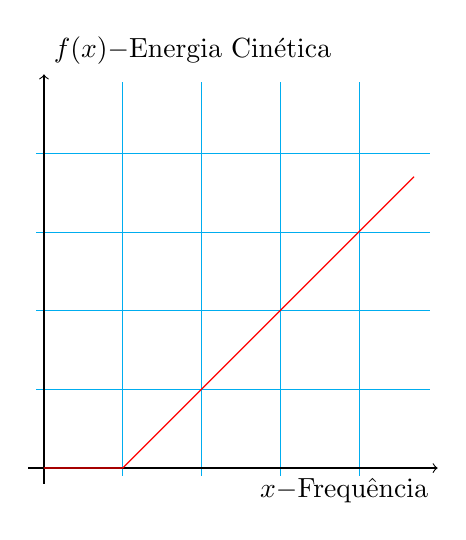
\begin{tikzpicture}[scale=1]
	\draw[very thin,color=cyan] (-0.1,-0.1) grid (4.9,4.9);

	\draw[->] (-0.2,0) -- (5,0) node[below left] {$x-$Frequência};
	\draw[->] (0,-0.2) -- (0,5) node[above right] {$f(x)-$Energia Cinética};
	\draw[color=red,mark=x,smooth] (0,0) -- (1,0) -- (4.7,3.7) ;

\end{tikzpicture}
\end{center}
\caption{Gráfico Energia cinética vs. Frequência}
\label{kinect_freq}
\end{figure}

No entanto, existe uma frequência crítica para cada metal, $f_0$, abaixo da qual não são emitidos eletrons. Isto mostra que a energia cinética é igual à frequência luz multiplicada por uma constante (isto é, o declive da linha) Essa constante é chamada constante de Plank e é dada pelo símbolo h.

\begin{equation}\label{const_plank}
	h= 6.63\cdot 10^-34 J\cdot s 
\end{equation}

Assim é possível escrever uma equação para a energia cinética do eletron emitido.

\begin{equation}
	E_c= h\cdot f - h\cdot f_0
\end{equation}

Este resultado não é consistente com a teoria da luz como uma onda. Uma explicação que é consistente com essa imagem é que a luz vem em pacotes discretos, chamados fótons, e cada fóton deve ter energia suficiente para ejetar um único elétron. Caso contrário, nada acontece. Assim, a energia de um único foton é:

\begin{equation}
	E_f=hf
\end{equation}